\section{Equivalência de Recursos}
\label{sec:equivalenciaRecursos}

O conceito de equivalência de recursos refere-se a situações em que recursos distintos podem ser trocados sem perda de função na tarefa sendo executada. Considere o seguinte exemplo:

\begin{quote}
	Lucas estava brincando com seu carrinho, quando uma das rodinhas se quebrou. Entristecido, ele procurou por seu pai, que, ao ver a aflição de seu filho, resolveu ajudar. Recolheu uma garrafa PET que estava por perto, desenroscou sua tampinha e a colocou no lugar deixado pela rodinha estragada. Tamanha foi a felicidade de Lucas ao poder voltar a brincar com o seu carrinho.
\end{quote}

O exemplo, apesar de lúdico, apresenta uma situação clara de equivalência entre recursos. Tanto a roda do carrinho como a tampa de garrafa possuem características específicas que as diferem e as individualizam, como material, valor, peso e cor. Além disto, ambas possuem objetivos principais distintos, uma é fechar enquanto a outra é proporcionar mobilidade. Apesar disto, ambas possuem uma função em comum: são capazes de rodar. Sendo esta a função que o carro de brinquedo necessita para o seu funcionamento, os dois objetos tornam-se equivalentes para esta tarefa.

É exatamente esse o sentido ao se afirmar que dois recursos são equivalentes. Um não precisa ser igual ao outro, mas apenas possuir uma característica que, em determinado momento, possibilite a intercambialidade. Seria possível, por exemplo, utilizar um \emph{joystick} como um dispositivo apontador e, a qualquer momento, substitui-lo por um \emph{laser pointer} de forma que os serviços necessários continuassem sendo providos. Repare que tais dispositivos, assim como a rodinha e a tampinha, são bastante diferentes em diversas de suas características, mas ainda assim são capazes de fornecer serviços iguais, como mover uma seta pela tela.

Tomando o caso anterior, caso uma aplicação necessite apenas da capacidade de indentificar localizações em uma tela, um apontador seria suficiente. Neste caso ao se buscar por apontadores no ambiente teríamos como resposta todos os dispositivos equivalentes nesta função (como \emph{mouses}, \emph{joysticks}, \emph{laser pointers} e \emph{trackpads}). Mas no caso de uma aplicação que necessite de saber dos movimentos do usuário (como o gesto de \emph{pinch-zoom}, pinça com os dedos) apenas o \emph{trackpad} seria adequado. Para que isto seja possível é necessário conhecer como é realizado o cálculo de equivalência entre eles.

\subsection{Cálculo de Equivalência}

Para que determinado recurso seja equivalente a outro, deve-se garantir que as 3 regras a seguir sejam sempre respeitadas. Para tal, admita que a notação $A \implies B$ denote que um recurso A é equivalente a um recurso B.

\begin{comment}
\begin{enumerate}
	\item $R1 \implies R2$;
	\item $R2 \implies R3$;
	\item $R1 \implies R3$.
\end{enumerate}

\begin{figure}[ht]
	\center
	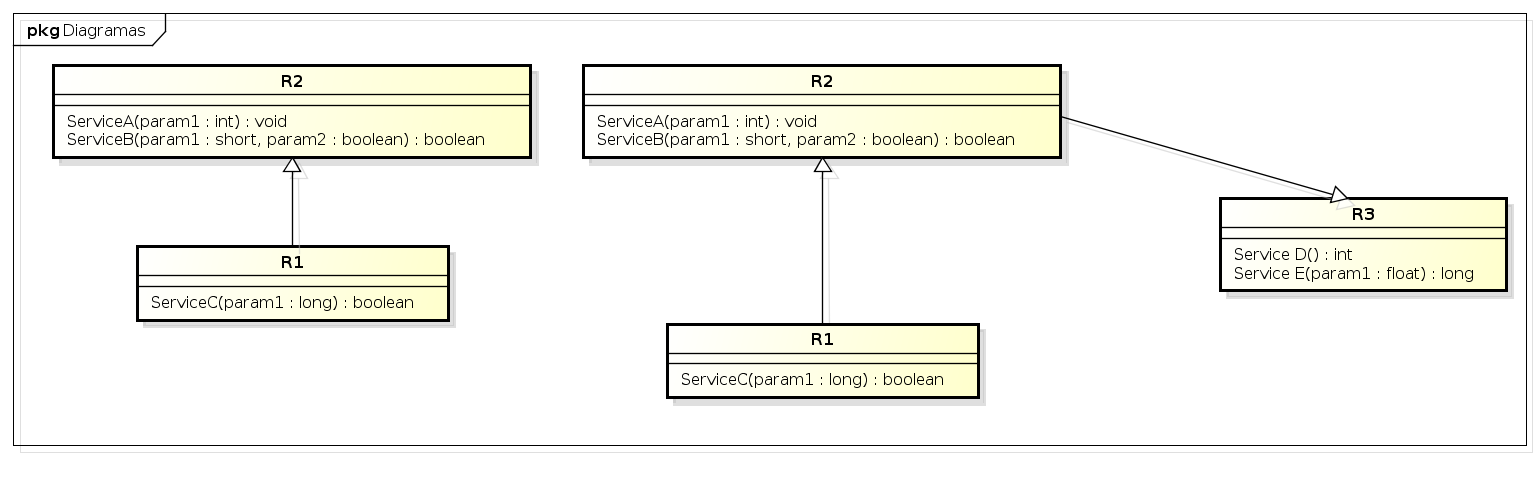
\includegraphics[scale=0.39]{imagens/calculoDeEquivalencia}
	\caption{Cálculo de equivalência: exemplo de recursos equivalentes.}
	\label{fig:calculoDeEquivalencia}
\end{figure}
\end{comment}

\begin{enumerate}
	\item Consistência de serviços

		Seja $R1 \implies R2$. Dessa forma, os serviços providos por R2 devem existir em R1. Observe que tal obrigação não impede que R1 contenha outros serviços desconhecidos por R2. Caso todos os serviços em R1 sejam iguais aos serviços em R2, tais recursos são iguais.
	\item Consistência de interface

		Seja $R1 \implies R2$. As interfaces dos serviços providos por R2 que também estão em R1 devem ser idênticas. Isso implica em dizer que os nomes dos serviços devem ser iguais, bem como os seus parâmetros.

		Parte-se do princípio que não existirá interesse em camuflar um serviço malicioso ao expor uma interface compatível com a equivalência.
	\item Refência circular

		Para a ocorrência de equivalência, é necessário a existência de uma classe inicial, à qual outros recursos possam se afirmar equivalentes. Neste caso, é necessario que não hajam ciclos nessas referências, de tal forma que seja possível encontrar a classe original.

		Por definição, são necessárias pelo menos duas classes distintas para a possibilidade de ocorrência de uma referência circular.
\end{enumerate}

Desta forma a relação de equivalência é:

\begin{itemize}
	\item Reflexiva: $R1 \implies R1$;

	\begin{itemize}
		\item Prova \\

		Sejam R1 e R2 recursos quaisquer tais que $R1 = R2$. Considere que S(X) represente o conjunto de serviços contidos no recurso X, que S($X \cap Y$) represente o conjunto resultante da intercessão dos serviços existentes em X e Y e que I(S(X)) seja o conjunto de interfaces dos serviços presentes em X. Logo: \\
		
		\begin{enumerate}
			
			\item $S(R1 \cap R2) = S(R2)$; \\
			\item $I(S(R1 \cap R2)) = I(S(R2))$; \\
			\item A quantidade de recursos distintos envolvidos é menor do que 2. Portanto não existe referência circular.
		\end{enumerate}
		\begin{flushright}$\Box$\end{flushright}
	\end{itemize}
	
	\item Não-simétrica: se $R1 \implies R2$ e $R1 \neq R2$, então o inverso não é verdade;

	\begin{itemize}
		\item Prova \\

		Sejam R1 e R2 recursos quaisquer tais que $R1 \neq R2$. \\

		\begin{enumerate}
			\item $S(R2 \cap R1) \neq S(R1)$; \\
		\end{enumerate}

		Pela falha da primeira regra, percebe-se que o recurso R2 não é equivalente a R1.
		\begin{flushright}$\Box$\end{flushright}
	\end{itemize}

	\item Transitiva: se $R1 \implies R2$ e $R2 \implies R3$, então $R1 \implies R3$.

	\begin{itemize}
		\item Prova \\

		Sejam R1, R2 e R3 recursos quaisquer tais que $R1 \implies R2$ e $R2 \implies R3$ e $R1 \neq R2$, $R2 \neq R3$ e $R1 \neq R3$. \\

		\begin{enumerate}
			
			\item $S(R2 \cap R3) = S(R3)$. Mas $S(R1 \cap R2) = S(R2)$. Logo, $S(R1 \cap R3) = S(R3)$; \\
			\item $I(S(R2 \cap R3)) = I(S(R3))$. Mas $I(S(R1 \cap R2)) = I(S(R2))$. Logo $I(S(R1 \cap R3)) = I(S(R3))$; \\
			\item $S(R2 \cap R1) \neq S(R1)$, $S(R3 \cap R2) \neq S(R2)$ e $S(R3 \cap R1) \neq S(R1)$.
		\end{enumerate}
		\begin{flushright}$\Box$\end{flushright}
	\end{itemize}	
\end{itemize}

\begin{comment}
Para que um recurso R1 seja equivalente a um recurso R2, os serviços de R2 deverão estar presentes no conjunto de serviços de R1, mas R1 poderá ter outros serviços que não estão presentes em R2. Seja S(X), o conjunto de serviços do recurso X, então teríamos que $S(R1) \cap S(R2) = S(R2)$. 

\begin{figure}[ht]
	\center
	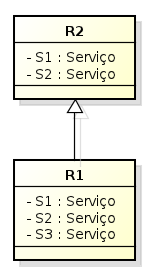
\includegraphics[scale=0.6]{imagens/equivalenciaDeRecursos}
	\caption{Exemplo de recursos equivalentes.}
	\label{fig:equivalenciaDeRecursos}
\end{figure}

Suponha uma situação em que $A \implies B$, $B \implies C$ e $C \implies A$, logo teríamos que $A \implies C$, o que seria uma relação circular, o que não faz sentido, pois concluiríamos que todos os recursos são iguais e não equivalentes. Devemos, portanto, garantir que não ocorra essa equivalência circular. Caso algum dispositivo queira registrar um novo \emph{driver} que cause essa inconsistência, devemos impedir que essa inconsistência possa ocorrer, ou então alertar o novo driver da ocorrência deste problema e não realizar seu registro.

\subsubsection{Consistência de Interface}

	A figura~\ref{fig:consistenciaInterface} mostra que o recurso R1 é equivalente ao recurso R3, mas embora possua um serviço de mesmo nome que o recurso R2,  seus parâmetros são diferentes, logo, não pode ser um mesmo serviço e os recursos não serão equivalentes..
	
	Para garantir que os recursos são equivalentes, devemos realizar três validações nas interfaces de cada serviço dos recursos:
	\begin{enumerate}
		\item Recurso:
			
			Os serviços devem pertencer ao mesmo recurso cujas classes padrões foram definidas anteriormente.
		
		\item Identificador do Serviço:

			Os serviços devem possuir os mesmos identificadores.

		\item Parâmetros:

			Os serviços devem possuir os mesmos parâmetros.
	\end{enumerate}

	Parte-se do princípio que não existirá interesse em camuflar um serviço malicioso ao expor uma interface compatível com a equivalência.

\begin{figure}[ht]
	\center
	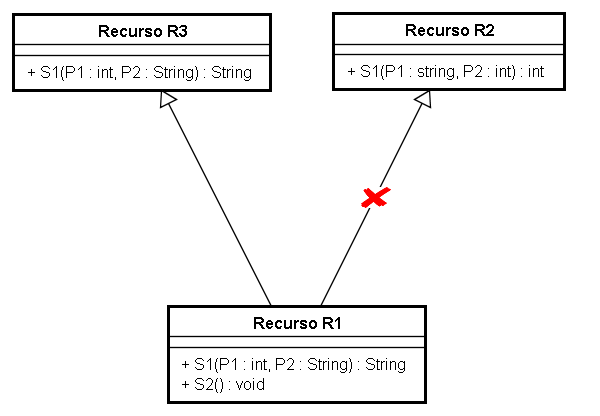
\includegraphics[scale=0.8]{imagens/consistenciaInterface}
	\caption{Exemplo de inconsistência de interface.}
	\label{fig:consistenciaInterface}
\end{figure}
\end{comment}

\begin{comment}
----------------------------------------- REVER ----------------------------------------- \\
Desta forma, faz-se necessária uma maneira de classificar tais recursos imersos nos mais variados dispositivos presentes no \emph{smart space} e regidos pelo \emph{middleware}. Essa classificação facilitará o desenvolvimento de novos \emph{drivers} para futuras aplicações, pois tornará possivel a definição de interfaces pré-estabelecidas que representem classes de recursos. Outra vantagem decorrente é a possibilidade de seleção de recursos equivalentes, caso o provedor originalmente selecionado esteja indisponível. \\
----------------------------------------- REVER -----------------------------------------

COLOQUEI NO COMEÇO DA PROPOSTA
\end{comment}

\subsection{Árvore de Recursos}

Cada uma das classes propostas servirá de raiz para uma árvore de recursos, ou seja, existirão diversas árvores, cada qual com outras classes agrupadas por funcionalidades formando um grafo desconexo. Dessa forma, toda definição de \emph{driver} ou declara explicitamente a quais outros \emph{drivers} ele é equivalente ou não declara nenhum e se torna uma nova raiz. Para tornar tal estrutura mais clara, considere a figura~\ref{fig:arvoreDeRecursos}. Observe a hierarquia formada a partir da classe padrão \emph{Pointer}. Ela é responsável por agrupar todas as classes de recursos capazes de prover serviços relacionados aos apontadores existentes, por exemplo, \emph{click} e \emph{scroll}. O mesmo acontece com as demais classes padrões. Essa estrutura onde cada subgrafo conexo forma uma árvore é importante, pois permite uma melhor organização lógica das classes relacionadas, além de permitir uma fácil navegabilidade entre elas.

\begin{figure}[ht]
	\center
	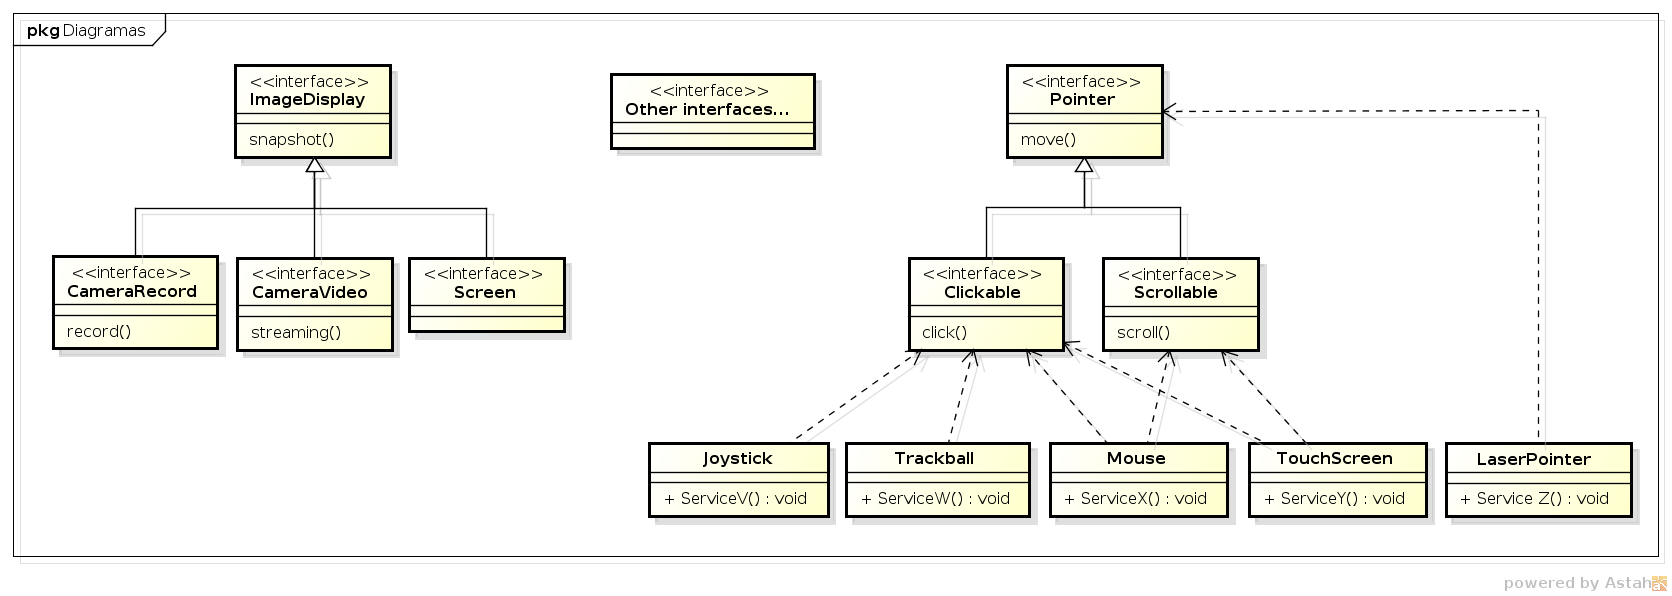
\includegraphics[scale=0.35]{imagens/hierarquiaDeRecursos}
	\caption{Exemplo da estrutura de árvores de recursos.}
	\label{fig:arvoreDeRecursos}
\end{figure}

Uma vez que tal estrutura esteja construída, para descobrir todos os recursos equivalentes a quaisquer classes presentes na árvore, basta tomar a subárvore cuja raiz é o elemento ao qual deseja-se obter seus equivalentes. Quanto mais próximo da raíz, mais genérico será o recurso, e à medida que se aproxima das folhas da árvore, mais específico será o recurso. Observe a figura~\ref{fig:tutorialDeEquivalencia} e imagine que seja necessário oferecer todos os recursos equivalentes à classe \emph{Clickable}. Ao se colocar tal classe como raiz de sua subárvore, torna-se fácil perceber que as classes \emph{Joystick}, \emph{Trackball}, \emph{Mouse} e \emph{TouchScreen} são suas equivalentes. A figura~\ref{fig:tutorialDeEquivalencia} mostra ainda situações de herança múltipla, em que \emph{Mouse} e \emph{TouchScreen} além de possuírem os serviços da classe \emph{Clickable}, possuem também serviços da classe \emph{Scrollable}.

\begin{figure}[ht]
	\center
	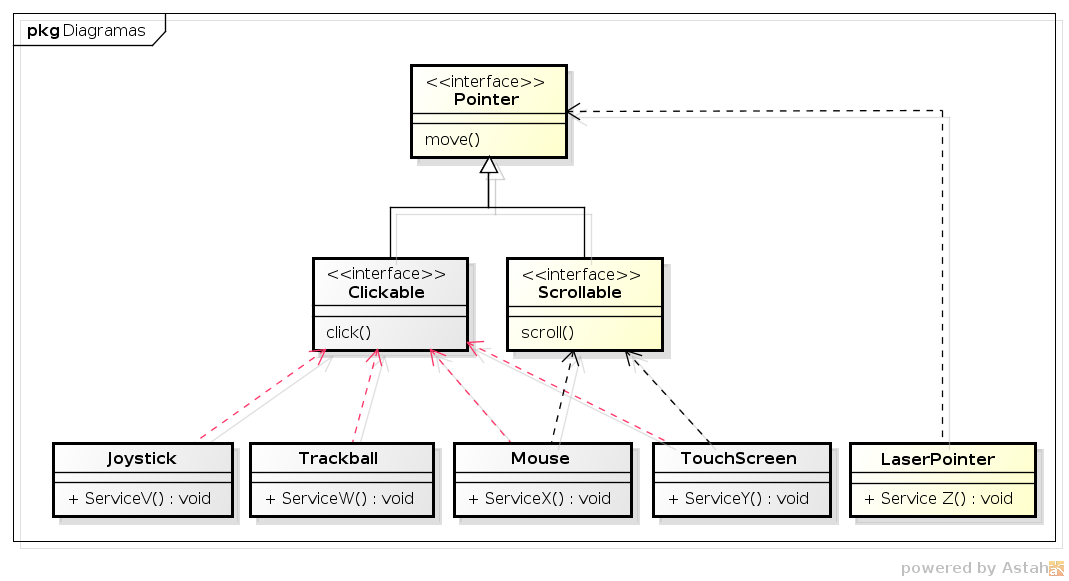
\includegraphics[scale=0.55]{imagens/tutorialDeEquivalencia}
	\caption{Exemplo de como se encontrar recursos equivalentes.}
	\label{fig:tutorialDeEquivalencia}
\end{figure}